\documentclass[conference]{IEEEtran}
\IEEEoverridecommandlockouts
% The preceding line is only needed to identify funding in the first footnote. If that is unneeded, please comment it out.
\usepackage{cite}
\usepackage{amsmath,amssymb,amsfonts}
\usepackage{hyperref}
\usepackage{graphicx}
\usepackage{textcomp}
\usepackage[T1]{fontenc}
\usepackage[utf8]{inputenc}
\usepackage{lmodern}
\usepackage[english]{babel}
\usepackage{todonotes}
\usepackage{algorithm}
\usepackage{algpseudocode}
\makeatletter
\renewcommand{\ALG@beginalgorithmic}{\small}
\makeatother

\usepackage{mathtools}
\usepackage{mathdots}
\usepackage{tikz-cd} 
\usepackage{wrapfig}
\usepackage{float}
\usepackage{quiver}
\usepackage{adjustbox}
\usepackage{stackengine,scalerel}
\newcommand\eye{\ensurestackMath{\stackinset{c}{}{c}{-.33pt}%
		{\bullet}{\bigcirc}}}
\newcommand\smallereye{\scalerel*{\eye}{x}}
\makeatletter
\newcommand{\removelatexerror}{\let\@latex@error\@gobble}
\makeatother


\newcounter{cases}
\newcounter{subcases}[cases]
\newenvironment{mycase}
{
	\setcounter{cases}{0}
	\setcounter{subcases}{0}
	\newcommand{\case}
	{
		\par\indent\stepcounter{cases}\textbf{Case \thecases.}
	}
	\newcommand{\subcase}
	{
		\par\indent\stepcounter{subcases}\textbf{ \>\>\>\> Subcase (\thesubcases)}
	}
}
{
	\par
}
\renewcommand*\thecases{\arabic{cases}}
\renewcommand*\thesubcases{\alph{subcases}}


\DeclareMathOperator*{\argmin}{argmin}
\DeclareMathOperator*{\pre}{^\bullet}
\usepackage{amsthm}
\usepackage{tikz}
\usetikzlibrary{cd}
\usetikzlibrary{petri,positioning}
\newtheorem{theorem}{Theorem}
\newtheorem{lemma}[theorem]{Lemma}
\newtheorem{remark}{Remark}
\newtheorem*{lemma*}{Lemma}
\newtheorem*{theorem*}{Theorem}
\newtheorem{definition}{Definition}

\newtheorem{example}{Example}

\def\BibTeX{{\rm B\kern-.05em{\sc i\kern-.025em b}\kern-.08em
		T\kern-.1667em\lower.7ex\hbox{E}\kern-.125emX}}
\begin{document}
	\title{Timed Alignments\\
		\thanks{Neha Rino was funded by the International Master's Scholarships Program IDEX of Université Paris-Saclay.}
	}
	
	\author{\IEEEauthorblockN{Thomas Chatain}
		\IEEEauthorblockA{\textit{LMF, ENS Paris-Saclay,}\\
			\textit{CNRS, Université Paris-Saclay, Inria} \\
			Gif-sur-Yvette, France\\
			\url{thomas.chatain@ens-paris-saclay.fr}\\
			ORCID 0000-0002-1470-5074}
		
		\and
		\IEEEauthorblockN{Neha Rino}
		\IEEEauthorblockA{\textit{LMF, ENS Paris-Saclay,}\\
			\textit{CNRS, Université Paris-Saclay, Inria} \\
			Gif-sur-Yvette, France\\
			\url{neha.rino@ens-paris-saclay.fr}}
	}
	
	
	\maketitle
	
	\begin{abstract}
		The subject of this paper is to study conformance checking for timed models, that is, process models that consider both the sequence of events in a process as well as the timestamps at which each event is recorded. 
		Time-aware process mining is a growing subfield of research, and as tools that seek to discover timing related properties in processes develop, so does the need for conformance checking techniques that can tackle time constraints and provide insightful quality measures for time-aware process models. 
		In particular, one of the most useful conformance artefacts is the alignment, that is, finding the minimal changes necessary to correct a new observation to conform to a process model.  
		In this paper, we set our problem of timed alignment and solve two cases each corresponding to a different metric over time processes. %For the first, we have an algorithm whose time complexity is linear both in the size of the observed trace and the process model, while for the second we have a quadratic time algorithm for linear process models. 
	\end{abstract}
	
	
	\begin{IEEEkeywords}
		Conformance checking, Alignments, Timestamps, Time Petri nets
	\end{IEEEkeywords}
	
	\section{Introduction} 
	%\subsection{Conformance Checking and Alignments} 
	Process mining studies vast systems through their event logs, and seeks to extract meaningful ways to model the underlying patterns or processes that govern the behaviour of the system in order to better understand it, or predict its future behaviour \cite{A16}.
	Once such a process model is obtained, it is natural to ask how one is sure the obtained model is a reasonable approximation of the system’s behaviour, especially given the issue of explainability in the domain of machine learning.
	Conformance checking is the art of judging the performance of a process model by relating the modelled behaviour and the observed behaviour of a process, without relying on the origin of the model \cite{CDSW18}.
	Observed behaviour comes in the form of traces in an \textit{event log}, a sequence of events that occur during the functioning of the system, while \textit{process models} are blueprints that describe what the underlying process of the system is expected to look like.
	Measures of how well a model reflects system behaviour include fitness, precision, generalisation, and simplicity.
	We often do not want the model to precisely generate all possible future system behaviour, but neither should it simply regurgitate the event log and accept no new system behaviours. 
	Hence, what is often sought is a process model that can, up to some acceptable error factor, approximate any reasonable future system behaviour. 
	
	In Arya Adriansyah's seminal thesis \cite{Adriansyah2014AligningOA}, we obtain the notion of an alignment, that is, the minimal series of corrections needed to transform an observed trace into the trace of the process model that most closely mimics it.  
	It can be computed using the synchronised product of the process model and a \emph{trace model} i.e. a simple model that captures exactly one event log trace. 
	This gives us a series of edits, usually insertions or deletions, that transform the observed trace  into a process trace.  
	%For our purposes we will use the term alignment to mean the process trace of the model that aligns closest to the observation, and how to transform this optimal execution to the observed one is clear depending on the edit moves available.
	Alignments thereby pinpoint exactly where inevitable deviations from expected behaviour occur, and the more distant the aligning word of a model is from its observed trace, the worse the model is at reflecting real system behaviour. 
	
	%\subsection{Time-aware Processes}
	
	Process models that do not seek to capture timing constraints can be represented using a variety of formal objects, including Petri nets and Business Process Mining Notation (BPMN).
	It is natural to want to study explicitly timed systems,	as by considering events along with their timestamps when mining processes, we can glean information about the minimum delay between two events, the maximum duration the system takes to converge upon a state, or check deadlines, all of which are highly relevant in real world applications \cite{Cheikhrouhou2014TheTP} \cite{Eder1999TimeCI} \cite{inbook}. 
	In addition, one may want to predict the timestamps of processes \cite{SSA11}. 
	Time-aware process mining seeks to study both what the underlying processes govern system behaviour are, and what time constraints they obey \cite{RMAW13} \cite{CRHA20}  \cite{AS21}. 
	In the process mining community, there are ways to use existing process model notation in order to denote time constraints. BPMN 2.0 comes equipped with \emph{timer events} and can record absolute, relative, and cyclical time constraints. 
	The main extensions to Petri nets that model time include time Petri nets, timed transition Petri nets, timed place Petri nets and timed-arc Petri nets. 
	For our purposes, we use \textit{time Petri nets} or TPNs, that is, Petri nets augmented with the ability to record and check the duration it takes to fire a transition once enabled, using which one can impose certain constraints on the relationships between the timestamps of different events. 
	While our discussion in this paper mainly centres time Petri nets, the notions of delay and stamp edits, the metrics defined and the problem statement can be adapted to suit these other models as well. 
	
	As time-aware process mining grows popular, new quality measures and conformance checking techniques must be developed that are sensitive to temporal constraints, but so far in the study of alignments as a conformance checking artefact, we notice that the process model used is never time-aware. 
	Traditionally, when one assumes the event logs are a list of words over a finite alphabet (the set of possible action labels), the problem of calculating the alignment has been extensively studied \cite{Adriansyah2014AligningOA} \cite{BCC21}. 
	The notion of distance used on these words used is usually either Hamming distance or Levenshtein's edit distance. 
Hence, for time-aware conformance checking, one requires a notion of distance over timed words, enabling us to measure how close two timed process traces are. Distances over timed words have been explored before, such as in \cite{ABD18} and \cite{CJM14}, both of have in common the notion of capturing the maximal difference between the timestamps attached to the same action label. In this paper we provide distinct distance functions that can reflect information about multiple timestamp discrepancies between timed words, and using them, we pose and solve the alignment problem for time-aware processes.

	%\medskip%\subsection{Three Distances, and Algorithms to Align them}
	
	In this paper, we start in Section \ref{sec:alignmentpb} by formally setting the alignment problem and, proposing three different distance functions over sequences of timestamps. 
	In Section \ref{mcg} we look at aligning under one of these distance functions, $d_t$, and give a quadratic time alignment algorithm in the case of a structurally restricted class of models (sequential causal processes).
	For all other types of models, in Section \ref{lpp} we present an encoding as a linear programming problem, albeit with slower worst-case time complexity. 
	Finally in section \ref{4} we study another distance function, $d_\theta$, which utilises the structure of the process model in its calculations, and we present a straightforward algorithm for solving the alignment in this case, whose time complexity is linear in the size of the causal process and the transition set of the model. 
	The second setting, and the notion of delay edits that we proposed, provide new insight into the nature of time processes and their properties.
	
	
	\section{Preliminaries}
	We represent events as pairs $(a,\tau)$ where $a \in \Sigma$ is the name of the action, and $t$ denotes the time at which said action was taken.
	
	\begin{definition}
		A timed trace is a sequence $\gamma \in (\Sigma \times \mathbb{R}^+)^*$ of timed events, seen as a timed word. 
	\end{definition}
	
	We will often ignore the action labels of timed words, i.e., deleting the projection $\pi_1$onto $\Sigma^*$, leaving just the timestamps, the projection $\pi_2$ onto $\mathbb{R}^{+*}$. 
	The timed process model we use here is a labeled time Petri net. 
	
	\begin{definition}[Labelled Time Petri Net] \label{tpn} A labeled \textit{time Petri net} (or TPN) is a tuple $N = (P, T, F, SI, \Sigma, \lambda, M_0, M_f)$, where $P, T$ are disjoint sets of places and transitions respectively,  $F \subseteq (P \times T) \cup (T \times P)$ is the flow relation,  $SI : T \rightarrow \mathbb{Q}^+ \times (\mathbb{Q}^+ \cup \{\infty\})$ is the static interval function, where $SI(t) = (Eft(t), Lft(t))$ such that $Eft$ stands for earliest firing time, and $Lft$ for latest firing time, $\lambda : T \rightarrow \Sigma$ is the labeling function, labeling transitions with actions from the action set $\Sigma$, and  $ M_0 , M_f: P \to \mathbb{N}$ are the initial and final markings. % of $N$. 
	\end{definition}
	
	Given a transition $t \in T$ we define the pre-set of $t$ as $\pre t = \{p \in P | (p, t) \in F\}$ and its post-set similarly is defined as $t \pre = \{p \in P | (t, p) \in F\}$, (the presets and post-sets of places are defined similarly). 
	A transition $t$ of a TPN is \textit{enabled} at marking $M$ iff $\forall p \in \pre t :  M(p) > 0$. 
	The set of all enabled transitions at a marking $M$ is denoted by \textit{Enabled(M)}. 
	
	A \textit{state} of a TPN $N = (P, T, F, SI, \Sigma, \lambda, M_0, M_f)$ is a pair $S = (M, I)$, where $M$ is a marking of $N$ and $I : Enabled(M) \rightarrow \mathbb{R^+}$ is called the \textit{clock function}. Every enabled transition hence has an implicit clock, measuring how long it has been since its most recent enabling. The initial state is $(M_0, \mathbf{0})$, where $\mathbf{0} $ is the zero function. 
	
	A transition $t$ can fire from state $S = (M, I)$ after a delay of $\theta \in \mathbb{R}^+$ post enabling 
	if $t$ is enabled at $M$, and $I(t) + \theta \in [Eft(t), Lft(t)]$ and for
	every other \(t'\) enabled at \(M\), $I(t') + \theta \leq Lft(t')$.
	%This last constraint encodes the notion of urgency, that is, if $t$ is enabled
	%at marking $M$ it must fire before its clock value reaches $Lft(t)$, unless
	%another transition disables it.
	This firing is denoted $(M, I)[t\rangle(M'', I')$ with the new state $(M'', I')$ defined as follows:
	$$M''(p) = \begin{cases}
		M(p) + 1 &  p \in t \pre \setminus \pre t\\
		M(p) - 1 & p \in \pre t \setminus t \pre\\
		M(p) & otherwise\\
	\end{cases}$$ 
	$$I'(t) =
	\begin{cases}
		I(t) + \theta & \textrm{If } t \in Enabled(M'') \cap Enabled(M')\\
		0 & \textrm{If } t \in Enabled(M'') \setminus Enabled(M')\\
	\end{cases}$$
	%Once a fireable transition $t$ is fired, the marking and clock function are both updated to reflect the firing, as defined below : %$M'$ as in the untimed case (subtracting one token from each preplace, and adding one token to each postplace), and the clock function $I$ is updated to $I'$ by increasing clock values by $\theta$ for any transition that was enabled at both $M$ and $M'$, setting clock values to 0 for any transitions newly enabled by $M'$ that were not enabled at $M$, and leaving clock values undefined for any transitions that are not currently enabled. 
	%% This is also denoted by $(M, I)[t\rangle(M'', I')$
	%An important feature of TPNs is the notion of urgency, that is, if $t$ is enabled at marking $M$ and has clock value $Lft(t)$, it must fire, or another transition must fire at the same instant disabling $t$.  
	
	%We need a notion of valid instances of processes the model wishes to recognise. This is why we equip our time Petri nets with a notion of a final marking. 
	A valid execution of the model begins at the initial state, fires a sequence of transitions %%(representing a series of activities occurring at certain times) and at the end of the firing sequence 
	and reaches $M_f$, with some clock function $I$. 
	
	\begin{definition}[Language of a TPN]
		A word $w = ((a_0, \tau_0), (a_1, \tau_1), \dots (a_n, \tau_n)) \in (\Sigma \times \mathbb{R})^*$ is in the language $\mathcal{L}(N)$ of the labeled TPN $N$ $\mathcal{L}(N)$ if there is a valid execution of the model such that there exists a sequence of transitions $(t_0, t_1 \dots t_n) \in (T, \mathbb{R^+})^*$ satisfying $(\lambda(t_0),\lambda( t_1), \dots,\lambda (t_n)) = w $ and they transform the initial state into a final one, that is, there exists some clock function $I$ on $M_f$, $(M_0, \mathbf{0}) [t_0, t_1, \dots t_n\rangle (M_f, I)$, where each $t_i$ is fireable at $\tau_i$. 
	\end{definition}
	
	\begin{example}\label{TPN}
		Consider the following example (adapted from \cite{AS21}) of a TPN $N$, modelling an airline refund office: \\
		\adjustbox{scale = 0.6}{
			
			\begin{tikzcd}
				& {} & \Huge\bigcirc & {\fbox{ec}} & \Huge\bigcirc & {} && {\fbox{pay}} \\
				\Huge\bigcirc & {\fbox{reg}} && {\fbox{et}} && {\fbox{dec}} & \Huge\bigcirc & {} & \Huge\bigcirc \\
				&& \Huge\bigcirc & {\fbox{{ct}}} & \Huge\bigcirc &&& {\fbox{rej}}
				\arrow["{[0, 1]}"{description, pos=0.2}, shift left=3, draw=white, from=2-2, to=1-2]
				\arrow[""{name=0, anchor=center, inner sep=0}, "{[2,2]}"{description, pos=0.1}, draw=white, from=2-4, to=1-4]
				\arrow["{[2,2]}"{description, pos=0.1}, draw=white, from=3-4, to=2-4]
				\arrow["{[2,4]}"{description, pos=0.1}, shift right=4, draw=white, from=2-6, to=1-6]
				\arrow["{[0,1]}"{description, pos=0.1}, draw=white, from=1-8, to=2-8]
				\arrow["{[0,0]}"{description, pos=0.1}, draw=white, from=3-8, to=2-8]
				\arrow[from=2-1, to=2-2]
				\arrow[curve={height=-12pt}, from=2-2, to=1-3]
				\arrow[curve={height=12pt}, from=2-2, to=3-3]
				\arrow[from=1-3, to=1-4]
				\arrow[from=1-4, to=1-5]
				\arrow[curve={height=12pt}, from=1-3, to=2-4]
				\arrow[curve={height=12pt}, from=2-4, to=1-5]
				\arrow[from=3-3, to=3-4]
				\arrow[from=3-4, to=3-5]
				\arrow[curve={height=-12pt}, from=1-5, to=2-6]
				\arrow[curve={height=12pt}, from=3-5, to=2-6]
				\arrow[from=2-6, to=2-7]
				\arrow[curve={height=-12pt}, from=2-7, to=1-8]
				\arrow[curve={height=12pt}, from=2-7, to=3-8]
				\arrow[curve={height=12pt}, from=3-8, to=2-9]
				\arrow[curve={height=-12pt}, from=1-8, to=2-9]
				\arrow["{[0,2]}"{description, pos=0.2}, draw=white, from=1-4, to=0]
			\end{tikzcd}
		}
		\\
		
		The action labels are as follows : Register request (reg), Examine thoroughly  (et), Examine casually (ec), Check ticket (ct), Decide (dec), Pay (pay), and Reject (rej). 
		
		The firing sequence $(reg, 1) (ec, 2)(ct, 3)(dec, 7)(rej, 7)$ is a valid execution of $N$. The initial marking only has $reg$ enabled, and registering the request at time $1$ updates the marking by removing the token from $reg$'s preplace and filling its two post-places, thereby enabling $ec, et, \textrm{ and } ct$. Now $ec$ fires at $2$, satisfying the constraint, filling one preplace of $dec$. Then $ct$ fires, having been enabled for $2$ units of time. Now, finally, $dec$ is enabled, and fires after $4$ units of having been enabled, and $rej$ is fired immediately after. 
	\end{example}
	
	Now we will build some vocabulary to help us talk about individual executions of timed words on TPNs, that take the form of branching paths. Much like runs of finite automata, causal processes are a way to unroll an execution of a Petri net, each element of $B$ being a copy of a place being visited by a token (so the same place if revisited will have multiple copies in $B$) and $E$ is the analogous object for copies of transitions fired in the original net. The partial order $G$ captures the copies of flow arcs in the original net, and hence it captures the causal relationships between different transitions and places during an execution. 
	%These correspond to runs in nondeterministic automata, but in this setting every configuration is a set of token-filled places, so to represent a particular execution we use what we define below as causal processes. 
	
	\begin{definition}[Causal Net] \label{cn}
		A \textit{causal net} $CN = (B, E, G)$ is a finite, acyclic net where 
		$\forall b \in B : |b \pre| \leq 1 \wedge | \pre b| \leq 1$. \linebreak $B$ (conditions) and $E$ (events) are the vertices, and $G$ denotes the edges. 
	\end{definition}
	
	%This can be viewed as the original Petri net itself, but every time a place is revisited, it is copied afresh to ensure that the execution only ever moves forward. 
	Multiple elements of $B$ or $E$ map to the same element in $P$ or $T$ respectively, a notion that is expressed via the map $p$ defined below. Let $Min(CN)$ is the set of vertices of $CN$ that are minimal under the $G$ pre-ordering
	
	\begin{definition}[Homomorphism] \label{hom}  Let $N$ be a TPN with place set $P$ and transition set $T$, and ${CN = (B, E, G)}$ be a causal net. 
		A mapping $p : B \cup E \rightarrow P \cup T$ is a \textit{homomorphism} if $p(B) \subseteq P$,  $p(E) \subseteq T$ and $\forall e \in E$ the restriction of $p$ to $\pre e$ is a bijection between $\pre e$ and $\pre p(e)$, the restriction of $p$ to $e \pre $ is a bijection between $e \pre $ and $p(e) \pre $ and the restriction of $p$ to $Min(CN)$ is a bijection between $Min(CN)$ and $Supp(M_0)$. 
	\end{definition}
	
	\begin{definition}[Causal Process]\label{cp} A \textit{causal process} of a TPN is a pair $(CN, p)$ where $CN$ is a causal net and $p$ is a homomorphism from $CN$ to $TPN$. 
	\end{definition}
	\todo[inline]{Example of a CP here?}
	Using $p$, elements of $CN$ are identified with their corresponding \emph{originals} in the TPN, and as a result, any causal process corresponds uniquely to an untimed run on the untimed version of a given TPN. 
	
	\begin{definition}[Timing Function]\label{tau} A \textit{timing function} $\tau : E \rightarrow \mathbb{R}$ is a function from events of a causal process into time values. 
	\end{definition}
	
	\todo[inline]{Should this section be here?\\
          Thomas: I am not sure yet, but let's try here. I need it for Lemma~\ref{lemma:distances} at end of Section~\ref{sec:alignmentpb}.}
	\subsection{A Note on Sequential Causal Processes}
        \todo[inline]{If we keep this section here, then slightly adapt the text.}
	We take a moment to discuss the structurally restricted class of processes that our stamp only-algorithm works for, that is, causal processes whose graphical structure  is that of a straight line. 
	These reflect the executions of TPNs that do not have any branching points ($e \in E : |e \pre | > 1$) and naturally as a consequence, no points of synchronisation ($e \in E : |\pre e| > 1$). 
	This essentially reflects the executions of automata, allowing for exclusive branching ($p \in P : |p \pre| > 1$) and iteration (that is, cycles in the model) only. 
	It loses the ability to capture properties of a concurrent nature, as the run never splits into more than one token. 
	On the other hand, the $G$ preorder becomes total, so studying the language of this restricted class and the alignment problem over it becomes substantially simpler, and so we restrict our attention to this class for the next section. 
	
	\begin{example}\label{Branchingcp}
		Going back to the net $N$ in example \ref{TPN}, and the firing sequence we analysed then $$w = (reg, 1)(ec, 2)(ct, 3)(dec, 7)(rej,7)$$ 
		
		We now construct the causal process of this execution, and see that it is indeed branching, as the very first transition, $reg$, itself has two post-places, which violates the no branching condition $e \in E : |e \pre | \leq  1$. 
		\adjustbox{scale = 0.8}{
			\begin{tikzcd}
				\bigcirc & {\fbox{reg}} & \bigcirc & {\fbox{ec}} & \bigcirc & {\fbox{rej}} & \bigcirc \\
				&& {\fbox{ct}} & \bigcirc & {\fbox{dec}} & \bigcirc
				\arrow[from=1-1, to=1-2]
				\arrow[from=1-2, to=1-3]
				\arrow[from=1-3, to=2-3]
				\arrow[from=2-3, to=2-4]
				\arrow[from=1-3, to=1-4]
				\arrow[from=1-4, to=1-5]
				\arrow[from=1-5, to=1-6]
				\arrow[from=2-4, to=2-5]
				\arrow[from=2-5, to=2-6]
				\arrow[from=2-6, to=1-6]
				\arrow[from=1-6, to=1-7]
		\end{tikzcd}}
		
	\end{example}
	
	\begin{example}\label{Sequentialcp}
		On the other hand, when we look at the model $N'$ from example \ref{stamptoy} we see that  all the branching and joining happens at places rather than transitions, so its executions all have sequential causal processes, such as below causal process for the untimed word $w = reg \cdot check \cdot dec \cdot pay$. \\
					
			\adjustbox{scale = 0.6}{
				\begin{tikzcd}
					\Huge\bigcirc & {\fbox{reg}} & \Huge\bigcirc & {\fbox{check}} & \Huge\bigcirc & {\fbox{dec}} & \Huge\bigcirc & {\fbox{pay}} & \Huge\bigcirc 
					\arrow[from=1-1, to=1-2]
					\arrow[from=1-2, to=1-3]
					\arrow[from=1-3, to=1-4]
					\arrow[from=1-4, to=1-5]
					\arrow[from=1-5, to=1-6]
					\arrow[from=1-6, to=1-7]
					\arrow[from=1-7, to=1-8]
					\arrow[from=1-8, to=1-9]		
				\end{tikzcd}
			}
			\\
		This causal process is unrolled from the Petri net, exactly the way runs of finite state automata are simple paths over the graph of the automaton. We throughout assume that wherever needed, such a causal process can be obtained via breadth-first search. 
	\end{example}

	\section{The Alignment Problem in Timed Settings}\label{sec:alignmentpb}
	The alignment problem, given a trace from an event log and a process model, involves finding a valid execution of the model that is closest to the trace under some metric.
	
	\begin{definition}[The General Alignment Problem]
		Given a process model $N$ denoted by a TPN and a timed trace $\sigma$ we wish to find a timed word $\gamma \in \mathcal{L}(N)$ such that $d(\sigma, \gamma) = \min_{x \in \mathcal{L}(N)} d(\sigma, x)$ for some distance function $d$ on timed words. 
		
	\end{definition}
	
	In the untimed setting, this is viewed as a problem of minimising cost over a series of edit moves, either insertions (\textit{model moves}) or deletions (\textit{trace moves}). When aligning timed words, clearly there are two crucial aspects to the problem, which are, how one deals with deviations in the action labels themselves, versus how one deals with deviations in just the timing properties of the word i.e., the timestamps. The alignment problem has been extensively studied for the untimed case \cite{Adriansyah2014AligningOA} \cite{BCC21}, %and so, if we simply sought to align the action labels of the word to the underlying untimed Petri net, this is a solved problem, 
	but the timed setting is more complex. 
	
	\begin{example}
		Consider the process model of Example \ref{TPN} and an observed trace $(reg, 1) \cdot (ec, 2) \cdot (ec, 2) \cdot (ct, 3) \cdot (dec, 8) \cdot (rej, 8)$ . Clearly, one shouldn't examine casually twice so one of the $ec$'s is extraneous, and also, the $dec$ event fires too late, it should have waited at most four time units after the firing of event $ct$. 
		Secondly, consider an observed trace of the form $(reg, 1) \cdot (ec, 2) \cdot (ct, 3) \cdot (dec, 7) \cdot (rej, 8)$. The control flow run itself is valid, but with the timestamps, we notice that the last transition is invalid. We could either edit the $rej$ action to a $pay$ one and leave the timestamp alone, or, edit the timestamp to get $(rej, 7)$. 
		Timestamps are attached to the letters they belong to, so it is hard to compare firing event $rej$ at time $7$ versus firing event $pay$ at time $8$ as the time constraints on different events are often different. In this manner, it is not clear how meaningful it would be to define edit moves that transform timestamps that are attached to different tasks. 
	\end{example}
	
	This is why, we first restrict our attention to the case where the untimed part of $\sigma$ does match the model, that is to say, if $\pi_1(\sigma)$ has a valid causal process $(CN, p)$ over $N$. Clearly this case of the problem needs to be solved if the general timed alignment problem is to be solved, and we argue that this case is interesting and complex in its own right. 
	
	This ensures that we can compare the timing constraints on analogous parts of the process, and hence reason meaningfully about timing deviations from the model. This gives us the following problem : 
	
	\begin{definition}[The Purely Timed Alignment Problem]
		Given a process model $N$ denoted by a TPN and a timed trace $w$, with timing function $\pi_2(w) = \sigma$ and a valid causal process of the untimed part $\pi_1(w)$, we wish to find a valid timing function $\gamma$ such that $d(\sigma, \gamma) = \min_{x \in \mathcal{L}(N)} d(\sigma, x)$for some distance function $d$ on timing functions. 
		
	\end{definition}
	
	In sections \ref{sec:alignmentpb}, \ref{3} and \ref{4} of this paper, we will ignore the action labels of the words, i.e we assume the word $\sigma$ we wish to align comes with a valid causal process $(CN, p)$ of the model, and seek to find timing functions on said causal process that are both valid, and minimize distance to $\sigma$ under the metric of choice. 
	
	We shall revisit the general timed alignment problem in section \ref{align}, and show how our methods 
	%for solving the purely timed alignment problem 
	can be adapted using existing techniques to provide approaches for solving the general 
	%timed alignment 
	problem. 
	
	\subsection{Edit Moves on Timing Functions}
	Now we come to the problem of comparing two timing functions over the same causal process, and quantifying how close they are to each other. 
	
	Much like Levenshtein's edit distance, popularly used in the untimed case of the alignment problem, we view the definition of these distances as an exercise in cost minimisation over the set of all transformations between two words. 
	In order to formalise the same, we need to define what the valid edit moves of such a transformation could be. 
	%We define \textit{moves} as functions that map one timing function over $(CN, p)$ to another. 
	%What sort of functions are useful notions of transformation on a timed system? 
	
	\begin{example}
		Let us go back to example \ref{TPN}, and study the process model $N$ presented there. 
		Say we had the following words that did not fit the model, and we wished to analyse how best to modify them to fit them back into the model. 
		
		We start with $\sigma = (reg, 1)\cdot  (ct, 2)  \cdot (ec, 2) \cdot (dec, 6) \cdot (rej, 6)$. 
		One candidate for the closest valid execution would be $\gamma = (reg, 1)\cdot  (ct, 3)  \cdot (ec, 2) \cdot (dec, 6) \cdot (rej, 6)$, and it feels reasonable to say that the cost for aligning $\sigma$ to this $\gamma$ is 1. 
		A way to arrive at this conclusion is by noticing that on trying to execute $\sigma$'s firing sequence only the guard for $ct$ fails. If $ct$ were shifted to fire at 3 instead, the whole run would execute without a hitch. This sort of local, almost typographical error can often happen in systems, and it is the simplest kind to fix.  
		
		There is, however, another way to look at it. A closest valid timing function would try to preserve the positions of $reg$ and  $ec$ but the moment it tries to fire $ct$, $\sigma$ runs early. By pushing $ct$ forward, it should take longer for the decision to be made and the rejection to happen, as those events depended on the checking of the ticket being done first. 
		This causes a cascading chain of errors where if $ct$ is moved forward to fire at 3, to preserve the relative relationships between $ct$ and its successors, we get the trace $\gamma' = (reg, 1)\cdot  (ct, 3)  \cdot (ec, 2) \cdot (dec, 7) \cdot (rej, 7)$, and in this sense, $\gamma'$ is closer to $\sigma$ as it preserves more relative gaps. As we just knocked one event a little later by 1 unit, we can view this as a cost 1 edit too.  
		%, if we assume $e$ and $f$ only care about the relative durations or delays between activities
	
		This is a slightly more complex type of error, but it reflects the real life fact of cascading errors, and hence is an important type of edit to consider when diagnosing such cascading faults. 
	\end{example}
	
	Based on the above example, we  arrive at two types of moves. 
	
	We define a \textit{stamp move} as a move that translates the timing function only at a point, i.e., that edits a single element of the timing function $\tau$. 
	
	\begin{definition}[Stamp Move]
		Given a timing function $\gamma : E \to \mathbb{R}$, formally, we define this as : 
		
		$\forall x \in \mathbb{R}, e \in E : stamp(\gamma, x, e) =\gamma' $ where
		$$\forall e' \in E : \gamma'(e')  = \begin{cases}
			\gamma(e') + x & e' = e \\
			\gamma(e')& otherwise
		\end{cases}$$
		
	\end{definition}
	
	The next type of move we describe is the more novel and interesting \textit{delay move}. 
	Here, we seek to leverage the structure of the process model itself, by reflecting the causal relationships the pre-order $G$ causes. 
	If an event $e'$ is $G$-reachable from another, say $e$, that means $e$ is strictly in the causal history of $e'$ so changing $e$'s timestamp should have consequences for all of its causal descendents, while leaving any causally unrelated (non-$G$-reachable) events undisturbed. 
	Hence, a delay move at $e$ will preserve relative relationships between timestamps in the future, at the cost of shifting the timestamp of every causal descendent of $e$  (such as $e'$) by the same amount. 
	\begin{definition}[Delay Move]
		Given a timing function $\gamma : E \to \mathbb{R}^n$, we define a delay move applied to it as follows : 
		
		$\forall x \in \mathbb{R}, e \in E : delay(\gamma, x, e) = \gamma'$ where 
		$$\forall e' \in E : \gamma'(e') = \begin{cases}
			\gamma(e') + x & e' \geq_G e \\
			\gamma(e')& otherwise
		\end{cases}$$
		
	\end{definition}
	
	The cost of a move is the magnitude $|x|$ in the above definitions, and the cost of a sequence of moves is the sum of the costs of the moves. Let the set of all stamp moves on a causal process be called $Stamp$, and the set of all delay moves be called $Delay$. Armed with these definitions, three natural notions of distance can be constructed. 
	
	\begin{definition}[Stamp Only Distance : $d_t$]
		Given any two timing functions $\tau_1, \tau_2$ over the same causal process $(CN, p)$, we define the stamp-only distance $d_t$ as follows : 
		
		$d_t(\tau_1, \tau_2) = \min \{cost(m) | {m \in Stamp^*}, {m(\tau_1) = \tau_2}\}$
	\end{definition}

        \todo[inline]{Thomas: I introduced these notations which are used in the examples. Check that there is no mistake.}
        For sequential causal processes (Def.~\ref{Sequentialcp}), we abuse
        notations and write \(stamp(x, i)\) for \(stamp(\gamma, x, e_i)\), and
        \(delay(x, i)\) for \(delay(\gamma, x, e_i)\), where \(e_i\) denotes the
        \(i\)\textsuperscript{th} event in the sequence induced by the process.
	
	\begin{definition}[Delay Only Distance : $d_\theta$]
		Given any two timing functions $\tau_1, \tau_2$ over the same causal process $(CN, p)$, we define the delay-only distance $d_\theta$ as follows : 
		
		$d_\theta(\tau_1, \tau_2) = \min \{cost(m) | {m \in Delay^*}, {m(\tau_1) = \tau_2}\}$
	\end{definition}
	
	\begin{definition}[Mixed Moves Distance : $d_N$]
		Given any two timing functions $\tau_1, \tau_2$ over the same causal process $(CN, p)$, we define the mixed move distance $d_N$ as follows 
		\small	$$d_N(\tau_1, \tau_2) = \min \{cost(m) | {m \in (Stamp \cup Delay)^*}, {m(\tau_1) = \tau_2}\}$$
		
	\end{definition} 
	
	\begin{example}\label{stamptoy}
		Consider a simplification of our net from \ref{TPN}, collapsing checking the ticket and the examination steps into one $check$ step : 
			
			We first have the process model $N'$ : \\
			
			\adjustbox{scale = 0.6}{
				\begin{tikzcd}
					& {} && {} && {} &&{} \\
					\Huge\bigcirc & {\fbox{reg}} & \Huge\bigcirc & {\fbox{check}} & \Huge\bigcirc & {\fbox{dec}} & \Huge\bigcirc & {\fbox{pay}} & \Huge\bigcirc 
					\arrow["{[0, 1]}"{description, pos=0.2}, draw=white, from=2-2, to=1-2]
					\arrow["{[0,1]}"{description, pos=0.2}, draw=white, from=2-8, to=1-8]
					\arrow[from=2-1, to=2-2]
					\arrow[from=2-2, to=2-3]
					\arrow[from=2-3, to=2-4]
					\arrow[from=2-4, to=2-5]
					\arrow[from=2-5, to=2-6]
					\arrow[from=2-6, to=2-7]
					\arrow[from=2-7, to=2-8]
					\arrow[from=2-8, to=2-9]
					\arrow["{[2,4]}"{description, pos=0.2}, draw=white, from=2-6, to=1-6]
					\arrow["{[2,2]}"{description, pos=0.2}, draw=white, from=2-4, to=1-4]
				\end{tikzcd}
			}

		Now for this $N$, let the observed trace's timing function ${\sigma = (3, 4, 8, 9) \not \in \mathcal{L}(N)}$. 
		
		The best $d_t$ alignment for the example in the diagram below is $\gamma = (1,3,7, 8)$ with minimum cost $d_t(\sigma, \gamma) = 5$. 
		
		The best $d_\theta$ \todo{right?} %% $d_t=\theta$
                alignment for the example in the diagram below is also $\gamma = (1,3,7, 8)$, but this time with minimum cost $d_\theta(\sigma, \gamma) = 3$, evidenced by the move sequence $(delay(-2, 1)delay(+1, 2))$.
                %% \todo{explain abuse of notation: in the definition, \(delay\) and \(stamp\) have 3 parameters}
		
		And lastly, the best $d_N$ alignment for the example in the diagram below is also $\gamma = (1,3,7,8)$, the sequence of moves being one stamp and one delay move at the start, $m = stamp(-1, 1)delay(-1, 1)$, and now with minimum cost $d_N(\sigma, \gamma) = 2 < \min \{d_t(\sigma, \gamma), d_\theta(\sigma, \gamma)\}$. 
	\end{example}
	
        \todo[inline]{Thomas: I added here the three following simple
          properties, taken from sl. 22 of Thomas' slides at IRIF. WDYT?}
        \begin{lemma}
          \label{lemma:distances}
          Given any two timing functions $\tau_1, \tau_2$ over the same causal
          process $(CN, p)$, the following inequalities hold:
	  \begin{itemize}
          \item $d_N(\tau_1, \tau_2) \leq d_t(\tau_1, \tau_2)$
          \item $d_N(\tau_1, \tau_2) \leq d_\theta(\tau_1, \tau_2)$
          \item If $(CN, p)$ is a sequential causal process, then $d_\theta(\tau_1, \tau_2) \leq 2 d_t(\tau_1, \tau_2)$
          \end{itemize}
        \end{lemma}
        \begin{proof}
          The first two inequalities hold by construction of the three distances \(d_t\) \(d_\theta\) and \(d_N\).

          \todo[inline]{Thomas: Neha, you should check that my notations are consistent with the rest of the paper.}
          For the last one, observe that every sequence of stamp moves in a sequential process can be
          transformed into a sequence of delay moves as follows: each stamp move
          \(stamp(x, i)\) can be replaced by a delay move at \(delay(x, i\) immediately
          followed by another delay move \(delay(-x, i+1\) which compensates the
          effect of the first one on the events after \(i\). The total cost of
          these two delay moves is twice the cost of the original stamp move. (If
          the \(i\)\textsuperscript{th} event is the last one, then there is nothing to
          compensate.)
          For example, a \(stamp(+3, 2)\) move applied to the timing function
          $(3, 4, 8, 9)$ gives \((3, 7, 8, 9)\) at cost 3. As a replacement,
          a \(delay(+3, 2)\) move gives \((3, 7, 11, 12)\) and its effect on
          the last two timestamps can be compensated by a \(delay(-3, 3)\) move.
          The total cost for the two delay moves is 6.
        \end{proof}
	
	\section{Results and Algorithm : Stamp Edits}\label{3}
	\begin{lemma}[Stamp only distance : $d_t$]\label{manhattan}
		
		
		$d_t$ as defined above is equivalent to the \textit{Manhattan distance} or \textit{taxicab distance} between two points of $\mathbb{R}^n$, where $|E| = n$, say $\mathbf{t} = (t_1, t_2, \dots t_n) $ and $\mathbf{s} = (s_1, s_2, \dots s_n)$, defined as $$d_t(\mathbf{t}, \mathbf{s}) = \sum_{i = 1}^{n} |t_i - s_i|$$
	\end{lemma}
		\begin{proof}
		The way we see this is as follows. 
		Given a causal process $CN = (B, E, G)$ and two timing functions (not necessarily constituting valid timings) $\tau_1, \tau_2$, let $$d_t(\tau_1, \tau_2) = \sum_{e \in E} |\tau_1(e) - \tau_2(e)|$$
		This is both achievable by stamp only moves by doing the corresponding $\tau_1(e) - \tau_2(e)$ stamp move to the second word, and is the least cost any such stamp only path can take as Manhattan distance obeys the triangle inequality, and every stamp move results in a word at exactly the same Manhattan distance from its predecessor as the cost of said stamp move. 
		
	\end{proof}

	
	
	This lemma also allows us to restate the alignment problem for $d_t$, as we see below. 
	
	\subsection{Casting Alignment as a Linear Programming Problem}\label{lpp}
	The alignment problem in the stamp-only setting can be viewed as a problem of convex optimization, minimizing the stamp only cost from a fixed observed trace $\sigma$, which by Lemma \ref{manhattan} is $cost(\tau|_i) = \sum_{j = 1}^{i} |\tau_j - \sigma_j|$ over the set of valid timestamp series $\tau$ for the model $N$. 
	What remains is to show that the space of valid runs of the model is a convex set, as shown in \cite{BM82}. 
	%In this paper, the concept of a firing domain is proposed, that is, at each configuration of the time Petri net, the set of valid time intervals in which a transition enabled at that configuration can fire. Using these firing domains, states are grouped into state classes,which are sets of states with clock functions in the same firing domain, and for bounded time Petri nets there are finitely many such state classes. 
	%Calculating equivalence classes of the same, successively, till we find final configurations, gives a characterisation of the solution set of all valid timestamp series, and this is proved to be of the following form, which is a set of constraints defining a convex set. 
	
	Hence, we claim that using an efficient encoding of the target function using the firing domain formulation described above, the problem can be cast as a linear programming problem, and LPP solvers can solve this in good time in practice.  
	
	\begin{theorem}\label{convexset}
		Given a bounded TPN $N$, an observed trace $\sigma$, and its causal process $CN = (B, E, G)$, the alignment problem can be viewed as seeking the vector $(\gamma_1, \gamma_2, \dots \gamma_{|E|})$ that minimizes the quantity $\sum_{e \in E} |\gamma_e - \sigma_e|$ over the set $\gamma \in \mathcal{L}(N)$ which can be cast as a linear programming problem. %, i.e, $$\underset{\alpha - \beta \in \mathcal{C}, \alpha, \beta \geq 0}{\mathsf{minimize}} \hspace{0.5em} \alpha + \beta  $$
		
		%	Where $\mathcal{C}$ is a convex set. 
	\end{theorem}
	
		\begin{proof}
		Lemma 1 (General Form Lemma) of \cite{BM82} states that the firing domains of state classes for any bounded TPN may be expressed as solution sets of systems of inequalities of the following form :  $$\begin{cases}
			a_i \leq t(i) \leq b_i & \forall i \\ 
			t(j) - t(k) \leq c_{jk} & \forall j \neq k
		\end{cases}$$
		
		As $\gamma \in \mathcal{L}(N)$  this means it obeys the set of inequalities corresponding to the state class containing the final marking. Now, the above constraint is convex, so $\gamma$ varies over a convex set. As $\sigma$ is a constant vector, translation by it will keep the space convex, so $\gamma - \sigma \in \mathcal{C}$ for some convex set $\mathcal{C}$. 
		
		Now, we wish to minimize $|\gamma - \sigma|$, but it would be better to view this objective as a linear function. To this end we use a trick from \cite{BV2014} and use the following variable translation : $$\alpha, \beta \geq 0 : \alpha - \beta = \gamma - \sigma$$
		
		As defined above, $\alpha$ and $\beta$ are minimal when they are absolute values of the nonnegative and negative components of the vector $\gamma - \sigma$, respectively, i.e. when their sum is $|\gamma - \sigma|$. Our alignment problem can now be equivalently cast as $$\underset{\alpha - \beta \in \mathcal{C}, \alpha, \beta \geq 0}{\mathsf{minimize}} \hspace{0.5em} \alpha + \beta  $$
		\end{proof}

	
	%% \begin{remark}
		
		By the above theorem we see that the alignment problem for $d_t$ is easily cast as a linear progamming problem, and can be solved by any linear programming solver. 
		%% Hence it can be solved in polynomial average running time, but
		However this approach does not take into account the specific form of our problem, and LPP methods can be slow in the worst-case. 
		
		This bound is not necessarily tight, but either improving it or proving its tightness are left for future work. While the general case seems to be hard to solve efficiently, there is a subclass of process models for which the problem seems more tractable, and moreover, has a quadratic time solution. 
		

		\subsection{A Direct Algorithm for Sequential Models}\label{mcg}
		\subsubsection{The $g_i$ functions}
		We are given a process model $N$, an observed trace $\sigma$, and its underlying sequential causal process $CN = (B, E, G)$ with homomorphism $p$ for the untimed run of $\sigma$ on $N$. 
		We express the cost of aligning a prefix of $\sigma$ to some timing function $\tau$ on the truncation of the sequential causal process up to the $i$th transition, call it $cost$. 
		$$cost(\tau|_i) = \sum_{j = 1}^{i} |\tau_j - \sigma_j| = |\tau_i - \sigma_i| + cost(\tau|_{i-1})$$
		Observe that the minimum cost to align $\sigma$ depends on the sum of precisely two things, the cost of aligning the last stamp, and the minimum cost of aligning the $n-1$ length prefix of $\sigma$, in such a manner that the last two timestamps obey the last static interval constraint.  
		This suggests that the minimal cost of aligning prefixes of $\sigma$ to prefixes of the model can be recursively calculated as a function of the last timestamp in the alignment of a given prefix. 
		
		Let $g_i(d) = \min\{cost(\tau|_i) | \tau|_i \in \mathcal{L}^i(N) \wedge \tau_i = d\} $. 
		
		Now, the recursive relation $g$ functions obey is : 
		$$g_{i+1}(d) = |d - \sigma_{i+1}| + \min_{d-d' \in [a,b]} g_i(d')$$
		If we can calculate the family of functions $\forall i \leq n : g_i$ efficiently, then the minimal cost for aligning $\sigma$ to $N$ is simply $\min_{d} g_n(d)$. 
		
		\begin{figure}[!t]
				\centering 
				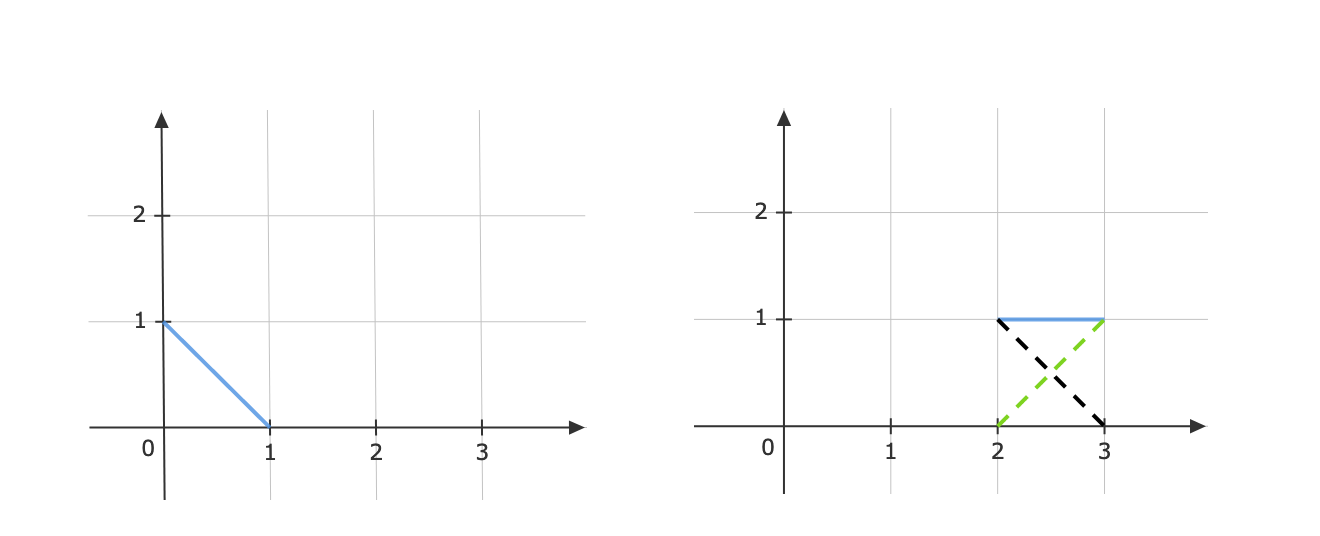
\includegraphics[width = 0.48\textwidth]{g12.png}
				
				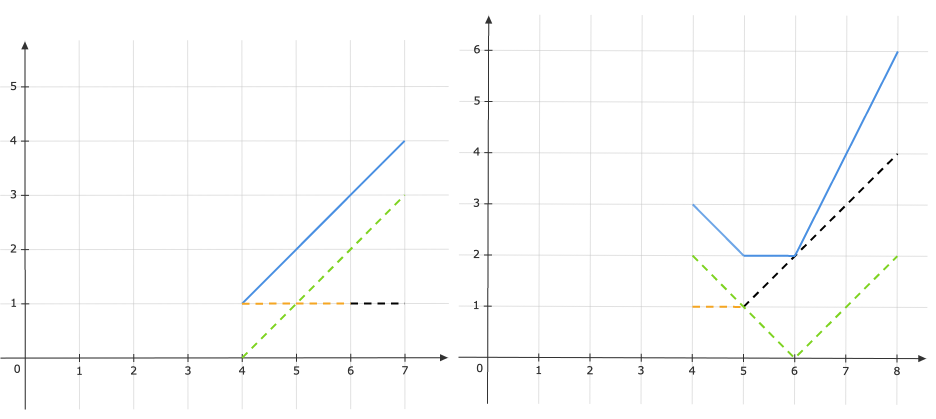
\includegraphics[width = 0.4\textwidth]{g34.png}
				\caption{Illustration of a run of the algorithm found in Example \ref{stampcomp}.}
			\end{figure}
		\begin{example}\label{stampcomp}
			
			We take a moment to look at an example of the computation of this family of functions on the model $N'$ from example \ref{stamptoy}, as it has a sequential causal process. 
			
				The observed trace is $\sigma = (reg, 1)\cdot (check, 2) \cdot (dec, 4) \cdot (pay, 6)$. 
			%%
			We begin to compute the family of functions $g_i$, and see that the cost of just aligning the $reg$ action as a function of its final timestamp is clearly $g_1(x) = |1-x|$ in the domain $[0,1]$.
			
			Now, we proceed to compute $g_2$.  
			The new domain is $[2,3]$, which is the same length as the previous one because the guard on the second transition is the point $[2,2]$. 
			Now, we want the sum of both the cost of aligning $check$ to $2$ in this domain, i.e, $|x-2|$ and the least cost of a corresponding alignment of $reg$ that obeys the $[2,2]$ clock interval condition, $\min_{x' - x \in [2,2]}g_1(x')$. 
			The first of these functions, i.e., the contribution of the last timestamp to the error, is pictured in figure 1 in green dashed lines. 
			The second component is pictured in black dashed lines, and is a translation of $g_1$, as $\min_{x' - x \in [2,2]}g_1(x') = g_1 - 2$. 
			
			We construct $g_3$ similarly, by summing the contribution of the last timestamp, $|x - 4|$, to  $\min_{x' - x \in [2,4]}g_2(x')$. 
			We now find an orange segment in the second component. This is used to demarcate any additional segments in  $\min_{x' - x \in [a_i, b_i]}g_{i-1}(x')$ not present in $g_{i-1}$, this is due to the laxness found in choosing a timestamp for $check$ given a timestamp for $dec$ as the current static interval constraint allows for multiple solutions. 
			Overall, we see that the effect of the $\min$ operation is to attach a segment with the same length as the $i$th static interval constraint, at the lowest point of $g_{i-1}$. 
			
			We continue similarly : The next black graph is a translation of the previous blue one, with an orange line segment or the same length as the next static interval constraint inserted at the lowest point, and the next green graph is $|x-\sigma_i|$ in the new domain, and summing these two gives the next blue graph. 
			As these are all piecewise linear graphs, summing is simply incrementing the slopes of all the segments of the black-orange curve by one if they're to the right of $\sigma_i$, and by minus one if they're to the left, and translating the height up as needed. 
			%Clearly the orange, black and green segments of the next graph are obtained like this, and $g_4$ is their sum. 
			
			The procedure for constructing $g_4$ is identical, and now finally we see that the minimum cost of $2$ is achieved in $g_4$ by paying at time 6. 
			Now, we know the contribution of the $(pay,6)$ to the error is 0, so this means we can deduce the corresponding value in $g_3$ must have been 2, achieved when $dec$ fires at 5. 
			We can backtrack in this manner to build an optimal alignment, such as in this case, $(reg,1)(check,3)(dec,5)(pay,6)$. 
			
			
		\end{example}
		\subsubsection{The Direct Stamp Algorithm}
		
		With this intuition, we present Algorithm \ref{StampAlgo} that progressively calculates the graphs of $g_i$ (represented as lists of segments, each characterised by their slopes and x-projections of endpoints) each round, and claim it is both correct and efficient. 
		The algorithm precisely executes the above procedure, where the subfunction \textsc{graphMin} takes $g_i(d)$ and outputs $$\min_{d-d' \in [a,b]} g(d') = \begin{cases}
			g(d-a) & l + a \leq d < m + a \\
			g(m) & m+a \leq d \leq m' + b \\
			g(d+b) & m' + b < d \leq h + b   \\
		\end{cases}$$ Which is to say, it inserts a flat segment of length $b-a$ at the lowest point of $g$. Subfunction \textsc{graphAddMod} takes $\min_{d-d' \in [a,b]} g(d')$ and adds $|d - \sigma_{i+1}|$ to it, i.e., adding the green component.  Lastly, the \textsc{backTrack} algorithm backtracks through the list of graphs $\{g_i\}_n$ constructed to reverse engineer a word that aligns with the minimal cost calculated. 
		
		\begin{figure}[!t]
			\removelatexerror
			\begin{algorithm}[H]
				\caption{$d_t$ Algorithm}
				\label{StampAlgo}
				\begin{algorithmic}
					\State \textbf{Input : }  $\sigma$, $SI$
					\State \textbf{Output : }  $cost = \min_{x \in \mathcal{L}(N)}{d_t(x, \sigma)}$, $\gamma \in \mathcal{L}(N)$ such that $d_t(\gamma, \sigma) = cost$
					
					\State \textbf{Object :} $graph = \{(left, slope, right) | graph[i].left = graph[i-1].right\}$
					
					\Procedure{StampOnlyAlgo}{$\sigma, SI$}
					\State Initialise System 
					\State $[a, b] \gets SI[i]$
					\State $graph \gets \{(a, 0, b)\}$
					\State \textsc{graphAddMod}($graph, \sigma[0]$)
					\State $graphlist \gets \{graph\}$
					\State $i \gets 1$
					\State $cost \gets |a - \sigma[0]|$
					
					\While{$i < |sigma|$}
					\State $[a, b] \gets SI[i]$
					\State \textsc{graphMin}($graph, a, b$)
					\State \textsc{graphAddMod}($graph, \sigma[i]$)
					\State $graphlist.append(graph)$
					\State $cost \gets cost + |a - \sigma[i]|$
					\EndWhile
					
					\State $i \gets 0$ 
					\State $s \gets graph[0].slope$
					
					\While{$graph[i].slope < 0$}
					\State $s \gets graph[i].slope$ 
					\State $cost \gets cost + s * (graph[i].right - graph[i].left)$
					\State $i \gets i + 1$
					\EndWhile
					
					\State $\gamma \gets \textsc{backTrack}(\sigma, graphlist, cost, SI)$
					\State \textbf{Return : } $cost, \gamma$
					\EndProcedure
				\end{algorithmic}
			\end{algorithm}
		\end{figure}
		
		\begin{theorem}\label{StampAlgoCorr}
			Algorithm \ref{StampAlgo} is correct, i.e., it outputs a valid execution
			$\gamma \in \mathcal{L}(N)$ which minimizes the distance $d_t(\gamma, \sigma)$
			to the trace $\sigma$.
		\end{theorem}
		
		\subsubsection{Correctness of Algorithm 1}
		
	Before we prove Theorem \ref{StampAlgoCorr}, we prove a small, relevant lemma. 
	
	\begin{lemma}\label{minpwc}
		For any convex piecewise linear function $g$, the following function $g'$ is also convex and piecewise linear. 
		$$g'(d) = \min_{d-d' \in [a,b]} g(d')$$
		
	\end{lemma}
	
	\begin{proof}
		We first note that if the domain of $g$ was $[l, h]$, the domain of $g'$ is $[l + a, h + b]$. 
		
		Say the leftmost minimum of $g$ (if $g$ has multiple minima they are all on the same flat line segment) is at $m \in [l,h]$. 
		For all $x \in [l + a, m+ a] $ and $x - y \in [a, b]$ and $y \in [l,h]$ implies $y \in [x-b+a, x-a] \cap [l, h] \subseteq [l, h] \cap [l-b+a m] = [l,m]$ meaning for each $x$, in the possible domain of $y$ $g(y)$ is a strictly decreasing function, hence  we have $$\forall x \in [l + a, m+ a] : \min_{x - y \in [a,b]} g(y) = g(x - a) $$
		
		Now, let the rightmost minimum of $g$ is $m'$. 
		For all $x \in [m + a, m' + b] $ and $x - y \in [a, b]$ and $y \in [l,h]$ implies $y \in [x-b, x-a] \cap [l, h]$, and $[x - b, x - a] \cap [m, m'] \neq \emptyset$. 
		Now, this means for each $x \in [m+a, m' + b]$ the domain of $y$ has a minimum of $g$, so we have $$\forall x \in [m + a, m'+ b] : \min_{x - y \in [a,b]} g(y) = g(m) $$
		
		Lastly, let  $x \in [m' + b, h + b] $ and $x - y \in [a, b]$ and $y \in [l,h]$. 
		This implies $y \in [x-b, x-a] \cap [l, h] = [m', h]$, so for each $x \in [m+a, m' + b]$ the domain of $y$ is in a region where $g$ is strictly increasing, so we have $$\forall x \in [m + a, m'+ b] : \min_{x - y \in [a,b]} g(y) = g(x+b) $$
		
		So we see that for any convex piece-wise linear function $g$, $$\min_{d-d' \in [a,b]} g(d') = \begin{cases}
			g(d-a) & l + a \leq d < m + a \\
			g(m) & m+a \leq d \leq m' + b \\
			g(d+b) & m' + b < d \leq h + b   \\
		\end{cases}$$
		
		Hence $g'$ is also convex and piecewise linear, and has at most one more linear segment than $g$. 
	\end{proof}
	

	We may now prove Theorem \ref{StampAlgoCorr}. 
	
		\begin{proof}
		We are given a process model $N$, an observed trace $\sigma$, and its underlying sequential causal process $CN = (B, E, G)$ with homomorphism $p$ for the untimed run of $\sigma$ on $N$.
		As discussed earlier, for sequential process models, we define $$g_i(d) = \min_{\tau|_i \in \mathcal{L}^i(N) \wedge \tau_i = d} cost(\tau|_i)$$
		
		This family of functions is seen to obey the following recursion: 
		
		$$g_{i+1}(d) = |d - \sigma_{i+1}| + \min_{d-d' \in [a,b]} g_i(d')$$
		
		If we can calculate the family of functions $\forall i \leq n : g_i$ efficiently, then the minimal cost for aligning $\sigma$ to $N$ is simply $$\min_{d} g_n(d)$$
		
		Hence to prove the correctness of Theorem \ref{StampAlgoCorr} we only need show that the auxiliary subfunctions called do indeed do their job correctly, as the main function just implements the recursion. 
		
		To this end, we first notice that the family of functions $g_i(d)$ are convex and piecewise linear. 
		This can be seen through induction : 
		
		Firstly $g_1(d) = |d - \sigma_1|$ so the base case is covered. 
		
		Now suppose $g_{i-1}$ is known to be convex and piecewise linear for some $i \geq 2$. 
		By Lemma \ref{minpwc} we see that $\min_{d-d' \in [a_i,b_i]} g_{i-1}(d')$  is also convex and piecewise linear, and so is $|d - \sigma_i|$ and both these properties are preserved by addition, so $g_i(d)$ must also be convex and piecewise linear. 
		
		Now that we have this result, our representation of the graph as a sequence of line segments, each represented as a triple (left x endpoint, slope, right x endpoint) is justified. 
		The y value of any graph $g_i$ can be back calculated because we know the value of the cost of the leftmost endpoint, it represents the word obtained by firing every transition at the earliest possible time. 
		
		Now subfunction \textsc{graphAddMod} is adding the point $\sigma_i$ if it is inside the domain of the function, and changing the slopes of the segments before $\sigma_i$ by subtracting one, and of those after $\sigma_i$ by adding one, which has the effect of adding the modulus component $|d - \sigma_i|$ to the previous graph. 
		
		Subfunction \textsc{graphMin} is even simpler, as Lemma \ref{minpwc} suggests all it does is translate the whole graph forward by $a$, and then translate the strictly increasing portion from $[m', h]$ by an addition $b-a$, adding an extra flat segment of length $b-a$ in between to keep the two portions of the function connected, and so on input $g(d), [a, b]$ it outputs $\min_{d-d' \in [a,b]}{g(d')}$. 
		
		Subfunction \textsc{backTrack} takes the minimum cost obtained by the calculation of the $g_n$ function, finds the value of $d$, ie $\gamma_n$ for which the minimum is achieved, and subtracts the cost aligning only the last place incurs, thereby finding the minimum cost for aligning the $n-1$ length prefix. 
		It then proceeds to do the same iteratively for each prefix, reverse-engineering a trace $\gamma$ for which the total minimum cost of aligning to $\sigma$ is achieved. 
		
	\end{proof}
	We include here pseudocode for the \textsc{backTrack} subfunction : 
	
	\begin{figure}[!t]
		\removelatexerror
		\begin{algorithm}[H]
			\caption{Backtrack to find the best word}
			\label{AuxFunc3}
			\begin{algorithmic}
				\State \textbf{Input : }  $\sigma$, $graphlist$, $cost$, $SI$
				\State \textbf{Output : }  $\gamma \in \mathcal{L}(N)$ such that $d_t(\gamma, \sigma) = cost$
				
				\For{$i = 0, i < |graphlist|$}
				\State Find $ylist[i]$, the $y$ values of $graphlist[i]$
				\EndFor
				
				\State $i \gets |sigma|-1$
				\While{$i \geq 0$}
				\State $[a, b] = SI[i+1]$ 
				\State Truncate $ylist[i]$ and $graphlist[i]$ so $ \gamma_{i+1} - x \in [a, b]$. 
				\State $k \gets $ \textsc{binarySearch}($ylist[i], cost$)
				\State $xsegment \gets graphlist[i][k]$
				
				\State $\gamma_i \gets xsegment^{-1}(cost)$
				
				\State $cost \gets cost - |\gamma_i - \sigma_i|$
				\State $i \gets i-1$
				\EndWhile
				
			\end{algorithmic}
		\end{algorithm}
	\end{figure}
	
		
		\begin{remark} Note that the subfunctions \textsc{graphMin} and  \textsc{graphAddMod} both run through the list of segments of the graph once each, and hence are linear in the sizes of their inputs, and Algorithm \ref{StampAlgo} calls each of these subfunctions once for each letter of the observed trace, each time on a graph with size linear in the current prefix.  
			So the cost calculation section of Algorithm \ref{StampAlgo} has quadratic time complexity in the size of the input. 
			
			The subfunction \textsc{backTrack} runs a binary search on each stored graph in $graphlist$ to find a trace in the language that does indeed give the minimum cost, letter by letter, and so overall takes $O(n \log(n))$ time, keeping the overall time complexity  $O(n^2)$ where $n = |\sigma|$.
		\end{remark}
		\todo[inline]{Should the example that shows $d_t$-alignment is not straightforward go here?}
		
		\begin{example}\label{dthard}
		In the simpler case of sequential causal processes it might not seem obvious why aligning under $d_t$ should require such global analysis and quadratic time to perform. While we do not present a proof of hardness here, a modification of our running example might show how aligning under $d_t$ is unlikely to be doable by some sort of greedy or locally optimising algorithm. Consider a third net, $N''$ that has the same actions as $N'$ but the constraints on them are different. 
					
			\adjustbox{scale = 0.6}{
				\begin{tikzcd}
					& {} && {} && {} &&{} \\
					\Huge\bigcirc & {\fbox{reg}} & \Huge\bigcirc & {\fbox{check}} & \Huge\bigcirc & {\fbox{dec}} & \Huge\bigcirc & {\fbox{pay}} & \Huge\bigcirc 
					\arrow["{[0, 50]}"{description, pos=0.2}, draw=white, from=2-2, to=1-2]
					\arrow["{[0,50]}"{description, pos=0.2}, draw=white, from=2-8, to=1-8]
					\arrow[from=2-1, to=2-2]
					\arrow[from=2-2, to=2-3]
					\arrow[from=2-3, to=2-4]
					\arrow[from=2-4, to=2-5]
					\arrow[from=2-5, to=2-6]
					\arrow[from=2-6, to=2-7]
					\arrow[from=2-7, to=2-8]
					\arrow[from=2-8, to=2-9]
					\arrow["{[0,0]}"{description, pos=0.2}, draw=white, from=2-6, to=1-6]
					\arrow["{[0,0]}"{description, pos=0.2}, draw=white, from=2-4, to=1-4]
				\end{tikzcd}
			}
			
			Let $\sigma = (reg, 0)(check, 0)(dec, 100)(pay,100)$ be an observed trace.
			Naively starting from the beginning, one might be tempted to construct the aligning trace $\gamma_{loc} = (reg, 0) (check, 0)(dec, 0)(pay, 0)$, but, the obvious best choices at the start of the trace incur heavy costs towards the second half, giving a total distance of $d_t(\sigma, \gamma_{loc}) = 200$. 
			
			A better choice would in fact be  $\gamma_{glob} = (reg, 50) (check, 100)(dec, 100)(pay, 100)$, as despite being very counter-intuitive at the start, it aligns better for the latter half of the trace, giving a total distance of $d_t(\sigma, \gamma_{glob}) = 150$. 
			
			A similar, two-sided version of this example could be constructed such that simply running the greedy check backwards on the trace will not help either, as the troublesome part of the execution is somewhere in the middle, and judging whether increasing costs initially can be made up for somewhere along the way is not easy. 

		\end{example}
		
		\section{Results and Algorithm : Delay Edits}\label{4}
		
		\subsection{Flows}
		
		Delay edits provide a new way of thinking about transformations over time-series, and inspire a new way of viewing timing functions over causal processes. 
		There is of course the standard definition, $\tau : E \to \mathbb{R}^+$ that assigns to each event a timestamp that records exactly when the event occurs. 
		
		Instead, thinking along the lines of durations between events occurring, we will often benefit from considering the following representation when speaking about delay moves, defined as to view a timed word not in terms of its absolute timestamps, but by the delays between them. 
		
		\begin{definition}[Flow Function]
			Given a causal process $(CN, p)$ over $N$, where $CN = (B, E, G)$, and a (not necessarily valid) timing function $\tau : E \to \mathbb{R}^+$, we first define the \textit{flow} function of $\tau$, $f_{\tau} : E \to \mathbb{R}^+$ such that 
			$$f_{\tau}(e) = \begin{cases} 
				\tau(e) & \pre \pre e = \emptyset\\
				\tau(e) - \tau(e') &e' \in   \pre \pre e,\\ & \tau(e') = \max\limits_{e'' \in \pre \pre e} {\{\tau(e'')\} \cup \{0\}}\\
			\end{cases}
			$$
			
		\end{definition}
		
		\begin{example}\label{wordandflow}
			Consider again the model $N$ in example \ref{TPN}.
			Say we want to align  $w = (reg, 1)(et, 2)(ct, 5)(dec, 6)(rej, 8)$ to $N$.  
			Consider the values the clock takes during a faulty ``execution'' $reg \to 1, et \to 1, ct \to 4, dec \to 1, rej \to 2$. This is the flow function. 
		\end{example}
		
		Note that $e'$ as defined here is the latest causal predecessor of $e$
		%, i.e., it is the firing of $e'$ that enabled $e$
		. 
		Hence, $f_\tau$ as defined produces exactly the time durations that the guards of each transition in the model checks, i.e. the clock function values during the run. 
		
		As defined, we see that if a word is in the language of the model, then its $f$ function maps events to values that lie within the event's static interval constraint. %% , and is perfectly aligned with the model. 
		This condition is unfortunately not sufficient due to urgency, but it is quite close to the exact condition necessary for a word to be in the language of a time Petri net. 
		
		Also note that given the underlying causal process and the resulting $f_\tau$, we can reconstruct $\tau$ quite straightforwardly as $\forall e \in E : \tau(e) = \sum_{e' \leq_G e} f_\tau(e')$.
		
		\begin{lemma}[Delay only distance : $d_\theta$]\label{manhattan2}
			
			$d_\theta$ as defined previously is equivalent to the following formulation directly using the flow function:
			$d_\theta(\tau_1, \tau_2) = \sum_{e \in E}|f_{\tau_1}(e) - f_{\tau_2}(e)|$.
		\end{lemma}	
				
	\begin{proof}
		By noting that delay moves on a trace $\tau$ translate exactly to stamp moves on $f_\tau$, we can deduce by the same argument as Lemma \ref{manhattan} that the distance function $d_\theta$ can be seen to be identical the manhattan distance on flow functions, i.e, the above formulation. 
	\end{proof}
	
		The flow function is hence a dual representation of timing functions, as if a timing function traditionally labels its transition nodes with timestamps, the flow function labels edges leading up to transitions with the duration since said transition was enabled. This gives us a new way to formulate the alignment problem in terms of minimising distance from the flow vector of $\sigma$. 
		
		
		\begin{example}
			Let us return to example \ref{wordandflow}. 
			Say we now wish to align  $w$ to $N$. We recall that we calculated its flow function to be $reg \to 1, et \to 1, ct \to 4, dec \to 1, rej \to 2$. 
			Pick the closest flow values in the model possible, naively, as illustrated bin Figure~{fig:DelayAlgo}.
			The resulting flow function is  $reg \to 1, et \to 2, ct \to 2, dec \to 2, rej \to 0$ From which we can reconstruct the closest word $u = (reg, 1)(et, 3)(ct, 3)(dec, 5)(rej, 5)$.
			
			Clearly if one tries to move any component of $u$'s flow function any closer to that of $w$, the word will no longer be in the language. 
			
		\end{example}
                \todo[inline]{Thomas: I have added an illustration for this example, taken from my slides.}
                \begin{figure}
\adjustbox{scale=0.6}{
\begin{tikzcd}
	& {} & \Huge\bigcirc & {\fbox{ec}} & \Huge\bigcirc & {} && {\fbox{pay}} \\
	\Huge\bigcirc & {\fbox{reg}} && {\fbox{et}} && {\fbox{dec}} & \Huge\bigcirc & {} & \Huge\bigcirc \\
	&& \Huge\bigcirc & {\fbox{{ct}}} & \Huge\bigcirc &&& {\fbox{rej}}
	\arrow["{1 \rightarrow 1}"{description, pos=0.2}, shift left=3, draw=white, from=2-2, to=1-2]
	\arrow[""{name=0, anchor=center, inner sep=0}, "{1 \rightarrow 2}"{description, pos=0.1}, draw=white, from=2-4, to=1-4]
	\arrow["{4 \rightarrow 2}"{description, pos=0.1}, draw=white, from=3-4, to=2-4]
	\arrow["{1 \rightarrow 2}"{description, pos=0.1}, shift right=4, draw=white, from=2-6, to=1-6]
%	\arrow["{[0,1]}"{description, pos=0.1}, draw=white, from=1-8, to=2-8]
	\arrow["{2 \rightarrow 0}"{description, pos=0.1}, draw=white, from=3-8, to=2-8]
	\arrow[from=2-1, to=2-2]
	\arrow[curve={height=-12pt}, from=2-2, to=1-3]
	\arrow[curve={height=12pt}, from=2-2, to=3-3]
	\arrow[from=1-3, to=1-4]
	\arrow[from=1-4, to=1-5]
	\arrow[curve={height=12pt}, from=1-3, to=2-4]
	\arrow[curve={height=12pt}, from=2-4, to=1-5]
	\arrow[from=3-3, to=3-4]
	\arrow[from=3-4, to=3-5]
	\arrow[curve={height=-12pt}, from=1-5, to=2-6]
	\arrow[curve={height=12pt}, from=3-5, to=2-6]
	\arrow[from=2-6, to=2-7]
	\arrow[curve={height=-12pt}, from=2-7, to=1-8]
	\arrow[curve={height=12pt}, from=2-7, to=3-8]
	\arrow[curve={height=12pt}, from=3-8, to=2-9]
	\arrow[curve={height=-12pt}, from=1-8, to=2-9]
%	\arrow["{[0,2]}"{description, pos=0.2}, draw=white, from=1-4, to=0]
\end{tikzcd}
	}
\caption{Illustration of Algorithm~\ref{DelayAlgo} for aligning $\sigma = (reg, 1)(et, 2)(ct, 5)(dec, 6)(rej, 8)$ to the model $N$ in example \ref{TPN}.
  Every label $a \rightarrow b$ on an action shows the delay \(a\) for the
  faulty ``execution'' guided by \(\sigma\), and the best corrected value \(b\)
  satisfying the time constraints in the model. From these corrected values we reconstruct the
  alignment $\gamma = (reg, 1)(et, 3)(ct, 3)(dec, 5)(rej, 5)$.
}
                  \label{fig:DelayAlgo}
                \end{figure}
		We could reason this way because $d_\theta$ allows one to locally edit traces without affecting membership in the language of the TPN, as both the firing rule and delay edits concern themselves only with the duration of time elapsed between a transition's enabling and its firing. 
		This relationship is especially clear in the following class of time Petri nets : 
		
			\begin{definition}[Extended Free Choice]\label{efc} A TPN is \textit{extended free choice} iff for all two transitions $t$ and $t'$, $\pre t \cap \pre t' \neq \emptyset$ implies $\pre t = \pre t'.$
	\end{definition}
	
	This class of TPNs ensure that the net is \textit{confusion-free}, that is, causally unrelated events cannot affect the fireability of other events. 
	\begin{figure}[!t]
			\removelatexerror
			\begin{algorithm}[H]
				\caption{Local $d_\theta$ Algorithm}
				\label{DelayAlgo}
				\begin{algorithmic}[1]
					\State \textbf{Input : }  $N$, $CN = (B, E, G), p$, $\sigma : E \to \mathbb{R}^+$
					\State \textbf{Output : }  $\gamma : E \to \mathbb{R}^+$ such that $\gamma$ is a valid timing function and $d_\theta(\gamma, \sigma)  \leq  {d_\theta(x, \sigma)}$ for all valid $x$ 
					
					\State $Curr = Min(CN)$
					\State $Enabled = \{t | \pre t \subseteq p(Curr)\}$
					\State $FD = \{(t, Eft(t), l, 0) | {t \in Enabled}, {l = \min_{\pre t' = \pre t}{Lft(t')}}\}$
					\State $Soon = \{{(t, eft, l, toe) \in FD} | {l+toe} \textrm{ is minimal in } FD\}$
					\While{ $E \neq \emptyset$} 
					\State Pick $(t, eft, l, toe) \in Soon, {t \in p(E)}$ 
					\State $E \gets E \setminus\{e | p(e) = t\}$
					\State $e \gets p^{-1}(t)$
					\State $Curr \gets \{Curr \setminus \{\pre e\}\} \cup \{e \pre\} $
					\State $f_{\gamma}(e) = \argmin_{x \in [eft, l]}|x - f_{\sigma}(e)|$
					\ForAll{$t' \in T \wedge \pre t' = \pre t$} 
					\State $Enabled \gets Enabled \setminus\{t'\}$
					\State $FD \gets FD \setminus\{(t', e', l', toe')\}$
					\EndFor
					\ForAll{$t' \in T \wedge t' \pre = t \pre$}
					\State $Enabled \gets Enabled \cup \{t'\}$
					\State $eft' \gets Eft(t')$
					\State $l' \gets \min_{\pre t'' = \pre t'}{Lft(t'')}$
					\State $toe' \gets toe + f_\gamma(e)$
					\State $FD \gets FD \cup \{(t', eft', l', toe')\}$
					\EndFor
					\State $Soon = \{{(t, eft, l, toe) \in FD} | {l+toe} \textrm{ is minimal in } FD \}$
					\EndWhile
					\State \textbf{return $\gamma$}
				\end{algorithmic}
			\end{algorithm}
			
		\end{figure}
	
		Hence, we present Algorithm \ref{DelayAlgo}, which minimizes the delay cost at each transition locally, while still overall ensuring membership in the language of the model. The main step in the algorithm is line 12, the rest just ensures validity. 
		
		\begin{theorem}\label{DelayAlgoCorr} Algorithm \ref{DelayAlgo} is correct, i.e., it outputs a valid execution
			$\gamma \in \mathcal{L}(N)$ which minimizes the distance $d_\theta(\gamma, \sigma)$
			to the trace $\sigma$.
		\end{theorem}

	
			

	
		\subsection{Correctness of Algorithm 2} 
			\subsubsection{Preliminaries for Delay Only Algorithm} 
	
	
	Now, in order to study \textit{timed} executions, we want to be able add a timing function to the causal process we defined above, thereby allowing us to record when different transitions are taken. 
	The following definitions, properties and theorems in this subsection cover the material developed in Aura and Lilius' article on Time Processes \cite{AL97}. 
	
	Given the definition of the timing function, we try to see how a time process unfolds. 
	First the initial events, that is, those enabled at $Min(CN)$ happen, and as each event occurs, new events are enabled and disabled. 
	In order to keep track of this, we first define the auxiliary Cut function that represents the effect of having all the events in a subset fire simultaneously (we only use Cut on sets of events that can concurrently fire), as defined below. 
	$$Cut(E') = (E' \pre  \cup Min(NS)) \setminus \pre  E'.$$
	
	Now we can define the  \textit{time of enabling} for a transition $t$ of a TPN in a set of conditions $B'$ of its causal process as $TOE(B', t) = $ $$ max(\{\tau(\pre b) | b \in B' \setminus Min(CN) \wedge p(b) \in \pre  t\} \cup \{0\})$$
	
	We must now verify that this timing function does indeed represent a valid execution that obeys all the static interval constraints, as below : 
	
	\begin{definition}[Valid Timing] \label{validt} A timing function $\tau$ is a \textit{valid timing} of the causal process iff 
		$$\forall e \in E : \tau(e) \geq TOE(\pre e, p(e) ) + Eft(p(e))$$
		$$\forall e \in E : \forall t \in Enabled (p(C_e)) : \tau(e) \leq TOE(C_e, t) + Lft(t)$$ 
		where $C_e = Cut(Earlier(e))$. 
	\end{definition}
	
	Here, checking every element of $C_e$ might seem unnecessary but in certain nets, complex dependencies between transitions can cause causally unrelated transitions to force transitions to fire or be disabled, due to urgency. 
	This phenomenon is known as confusion, and hence to guard against this, a timing function must check that it never leaves a section of the process behind, completing the firing or disabling of every event in $Earlier(e)$ before it can reason about the fireability of $e$. 
	
	\begin{definition}[Time Process] \label{tp} A \textit{time process} of a TPN $N$ is a triple $(CN, p, \tau)$ where $\tau$ is a valid timing of $(CN, p)$ which is a causal process of $N$. 
	\end{definition}
	
Note that for extended free choice time petri nets, in order to check for the validity of a timing function, checking all of $C_e$ as before is no longer necessary. 
	
	How do we construct a valid timing function on the fly? 
	Given a partial time process of a TPN, we want to be able to study the effect of firing particular transitions amongst the set of transitions currently enabled. 
	In order to do so, we notice the following class of transitions. 
	
	A transition $t$ is a \textit{choice} at $B' \subseteq B$ iff $B'$ is a co-set that maps injectively to places and $\pre t = p(B')$, and a choice is an \textit{extension} of the process iff $B' \subseteq Cut(E)$. 
	
	These transitions reflect exactly the transitions enabled at a particular moment in the evolution of the process. Either they must be fired or disabled, by the urgency condition. 
	
	Given the above, Aura and Lilius characterise a method by which one can build partial time processes inductively, building forward while maintaining the validity of the timing function, denoted as keeping the process complete with respect to the timing function : 
	
	\begin{definition} A causal process $(CN, p)$ of a TPN where $CN = (B, E, G)$ is said to be \textit{complete} with respect to a timing function $\tau$ iff for every extension transition $t$ of the process, $$\max\{\tau(e)| e \in E\} \leq TOE(Cut(E), t) + Lft(t).$$
	\end{definition}
	
	Now given this, the following theorem due to Aura and Lilius \cite{AL97} holds : 
	
	\begin{theorem}\label{thm35}
		Let $N$ be an extended free choice TPN and $(CN, p)$ a causal process of $N$, where $CN = (B, E, G)$. A timing function $\tau$ is valid iff the following criteria hold : 
		
		\begin{enumerate}
			\item$ \forall e \in E :  Eft(p(e)) \leq \tau(e) - TOE(\pre e, p(e))$
			\item $\tau(e) - TOE(\pre e, p(e)) \leq  \min \{Lft(t) | \pre t = \pre p(e)\}$
			\item $(CN, p)$ is complete with respect to $\tau$, i.e, for every extension transition $t$ of the process, $$\max\{\tau(e)| e \in E\} \leq TOE(Cut(E), t) + Lft(t)$$
			
		\end{enumerate}
	\end{theorem}
	

	\subsubsection{Proof of Theorem \ref{DelayAlgoCorr}}

	Now that we have defined all the requisite notions, we can continue with the proof of the correctness of Algorithm 2. 
	
	\begin{proof}
		By theorem \ref{thm35} proved in Aura and Lilius' article \cite{AL97}, we know that in order to ensure that this is a valid time process, we need only ensure three inequalities hold as the time process $\gamma$ evolves. 
		
		\begin{enumerate}
			\item$ \forall e \in E :  Eft(p(e)) \leq \gamma(e) - TOE(\pre e, p(e))$
			
			By definition $f_\gamma(e) = \gamma(e) - TOE(\pre e, p(e))$, and by line 6 of the algorithm the variable $eft$ is correctly initialised to store $Eft(p(e))$, and line 17 ensures the above inequality holds. 
			
			\item $\gamma(e) - TOE(\pre e, p(e)) \leq  \min \{Lft(t) | \pre t = \pre p(e)\}$
			
			In similar vein, line 6 also ensures that $l$ is initialised precisely to store $\min \{Lft(t) | \pre t = \pre p(e)\}$, and line 17 again enforces the left hand side to be less than $l$. 
			
			\item $(CN, p)$ is complete with respect to $\gamma$, i.e, for every extension transition $t$ of the process, $$\max\{\gamma(e)| e \in E\} \leq TOE(Cut(E), t) + Lft(t)$$
			
			At every point when assigning a timestamp to an event, it is ensured that it belongs to $Soon$, a set defined to contain only those enabled events that have the least value of $l + toe$, or, $TOE(Cut(E), p(e)) + Lft(p(e))$. 
			This ensures that whenever an event $e$ is assigned a timestamp $\gamma(e)$, for all extension transitions $t$  (which must either be causal descendents of $e$ or already enabled when $e$ was picked, thereby being in $Enabled$, by extended free choice) we know that $\gamma(e) \leq TOE(Cut(E), p(e)) + Lft(p(e)) \leq TOE(Cut(E), t) + Lft(t)$. 
			
			Hence, $(CN, p, \gamma)$ is a valid time process of $N$. 
			
		\end{enumerate}
		
		As for its optimality, we see that any other valid time process would have to obey the same inequalities, in particular for another valid timing function $\gamma'$ it would have to obey $$f_{\gamma'}(e) \in [Eft(p(e)), \min_{\pre t' = \pre p(e)}{Lft(t')}] = [a,b]$$ and hence at any event $e$ where $\gamma$ differs from $\gamma'$ it would have lower than or equal cost for that event as $$f_\gamma(e) = \argmin_{x \in [a, b]} |f_\sigma(e) - x|$$
		
		Hence, the algorithm is correct. 
	\end{proof}

		\begin{remark} Note that Algorithm \ref{DelayAlgo} runs through the events of the causal process $E$ exactly once, and each time runs through the set of currently enabled transitions, and the total set of transitions, and hence its time complexity is linear in the size of the input $|CN|$, and the size of the transition set, i.e, $O(|E||T|)$. 
		\end{remark}
		\section{The General Timed Alignment Problem} \label{align}
		
		Now that we have provided methods to tackle the purely timed alignment problem for two metrics, we return to the general timed alignment problem. As our examples throughout have reflected, the purely timed alignment problem does not so much ignore the action labels as assume that they do  not need editing. 
		As a result, one approach for solving the general timed alignment problem would be to begin by completely ignoring the timed aspect, and aligning only the action labels of the word $w$ and the process model $N$ (now reduced to the underlying untimed Petri net) using the $\mathbb{A}^*$ algorithm\cite{Adriansyah2014AligningOA}, which can be used to get a valid control flow, that is, a valid causal process. This, for us, is an untimed word $w'$ which can then be given a timing function based on that of $w$, %preserving timestamps wherever possible and 
		repeating or deleting timestamps for any insertion or deletion moves. This yields a valid causal process and a potentially invalid timing function over it, which is then cast as a purely timed alignment problem. 
		
		This approach is quite naive, as it may have a tendency to exaggerate the importance of action label errors. For example, consider the following scenario : 
		
		\begin{example}
			Consider the following net $N_3$: \\
			\adjustbox{scale=0.8}{
				\begin{tikzcd}
					\eye & {\fbox{a}} & \bigcirc & {\fbox{a}} & \bigcirc & {\fbox{a}} &\bigcirc \\
					& {\fbox{b}} & \bigcirc & {\fbox{a}} & \bigcirc & {\fbox{a}} \\
					\arrow[from=1-1, to=1-2]
					\arrow[curve={height=12pt}, from=1-1, to=2-2]
					\arrow[from=1-2, to=1-3]
					\arrow[from=1-3, to=1-4]
					\arrow[from=1-4, to=1-5]
					\arrow[from=1-5, to=1-6]
					\arrow[from=1-6, to=1-7]
					\arrow[from=2-2, to=2-3]
					\arrow[from=2-3, to=2-4]
					\arrow[from=2-4, to=2-5]
					\arrow[from=2-5, to=2-6]
					\arrow[curve={height=12pt}, from=2-6, to=1-7]
					\arrow["{[0,0]}"{description, pos=0.1}, draw=white, from=1-2, to=2-2]
					\arrow["{[0,0]}"{description, pos=0.1}, draw=white, from=1-4, to=2-4]
					\arrow["{[0,0]}"{description, pos=0.1}, draw=white, from=1-6, to=2-6]
					\arrow["{[100,100]}"{description, pos=0.1}, draw=white, from=2-2, to=1-2]
					\arrow["{[0,0]}"{description, pos=0.1}, draw=white, from=2-4, to=1-4]
					\arrow["{[0,0]}"{description, pos=0.1}, draw=white, from=2-6, to=1-6]
			\end{tikzcd}}
			\todo[inline]{Thomas: I left the \([100, 100]\) only on \(b\)
                          (it was originally on all the actions of the bottom
                          line). Right?}
			
			Now, let the observation be ${(a, 100)(a, 100)(a, 100)}$. 
			The alignment the above approach would provide is $(a, 0)(a, 0)(a, 0)$. 
			But if we assign even a tenth of the cost of action edits to timestamp edits, clearly the closer word in the language was $(b, 100)(a, 100)(a, 100)$. 
		\end{example}
		\todo[inline]{How do we define a distance including action labels, without running into the problem highlighted in example 2?\\
                  Thomas: It does not solve the problem in Example 2. Depending
                  on the cost we assign to action edits, one or the other
                  alignment will be preferred. This is quite fair, I think. There is not even much to say about it.}
		The issue here is the tradeoff between timestamp edits and action label edits. A better approach would assign one cost $c_A$ to action edits and another $c_T$ to time edits, and seek to minimise their sum. A potential fix to our previous idea would be to essentially retain the above approach, but instead of just doing it for the best untimed alignment, take a selection of good untimed alignments (up to some allowable threshold), and try to align timestamps for each untimed candidate, and then minimise the total cost over this set. This alleviates some of the bias towards preserving action labels by allowing for small action deviations in case the timestamp alignment proves particularly cost efficient, but this is still a naive approach to the wider problem, and we hope to find better solutions in the future. 
		
		\section{Implementation}
		
		We have implemented the stamp only alignment algorithm in Python, available at \url{https://github.com/NehaRino/TimedAlignments}. This algorithm is quadratic in time complexity, and runs well in practice, as seen below 
		\centerline{
			\begin{tabular}{|c|c|c|c|}
				\hline
				Trace Length & 10 & 100 & 1000\\
				\hline
				Running Time (seconds) & 0.001 & 0.1 & 9.8 \\ 
				\hline
			\end{tabular}
		}
		

		
		\section{Perspectives and Conclusion}
		
		In this paper, we posed the alignment problem for timed processes, devised three metrics for studying alignments for timestamp sequences, and solved the purely timed alignment problem for the first two metrics proposed. As far as we know, this is the first step in conformance checking for time-aware process mining, and much further work can be inspired from this point. The alignment problem for the third metric $d_N$ is a first future direction. Secondly, for both metrics studied here the class of models for which the alignment problem was solved efficiently are structurally restricted (being sequential causal processes for $d_t$ and extended free choice time Petri nets for $d_\theta$) and it would be interesting to see how to broaden their scope to larger classes of process models.  Also, while the definitions of the metrics and problems presented here do readily adapt to other types of timed process models such as time transition/place Petri nets or timed-arc Petri nets, the methods for solving the problems may not. Thirdly, further investigation in the general timed alignment problem is necessary, as our proposed approach here is rather rudimentary and can certainly be improved. Lastly, there are a number of other conformance artefacts that can be set and studied in the timed setting, such as anti-alignments \cite{CBC21}, and one can better develop all such conformance checking methods to account for timed process models.
		%%mention g-algo specifically?
		\bibliographystyle{IEEEtran}
		\bibliography{Conformanceieee}

	

	
	
	
\end{document}







